% Full instructions available at:
% https://github.com/elauksap/focus-beamertheme



\newcommand*\circled[1]{
\tikz[baseline=(char.base)]{\node[shape=circle,draw,inner sep=2pt] (char) {#1};}
}

\newcommand{\quizV}{     
\begin{center}
     	\only<1>{\Huge{\circled{V}} \Huge{\circled{F}}}
        	\only<2->{\hspace{-4.6mm}\Huge{\color{green}{\circled{V}}} \Huge{\circled{F}}}
\end{center}
}
     
\newcommand{\quizF}{     
\begin{center}
  	 \only<1>{\Huge{\circled{V}} \Huge{\circled{F}}}
       	 \only<2->{\hspace{-4.6mm}\Huge{\circled{V}} \Huge{\color{red}{\circled{F}}}}
\end{center}}






\documentclass{beamer}
\usetheme{focus}
\usepackage{animate}

\title{GUIDA SICURA: Cap. Z}
\subtitle{uso ed equipaggiamento del veicolo}
\author{ACI Prima Porta}
\date{}
\titlegraphic{
	\vspace{1cm}
    	
\includegraphics[scale=0.89]{images/logo.jpg}
}

\begin{document}
\begin{frame}
        \maketitle
\end{frame}
    
% \begin{frame}{overview}
% \tableofcontents
% \end{frame}
% \section{Introduction}
    
    
    
\section{Documenti obbligatori}
    
    
\begin{frame}{Auto nuova?}
	Che fare? Che documenti servono?
    	\begin{figure}[ht!]
    		\centering
         		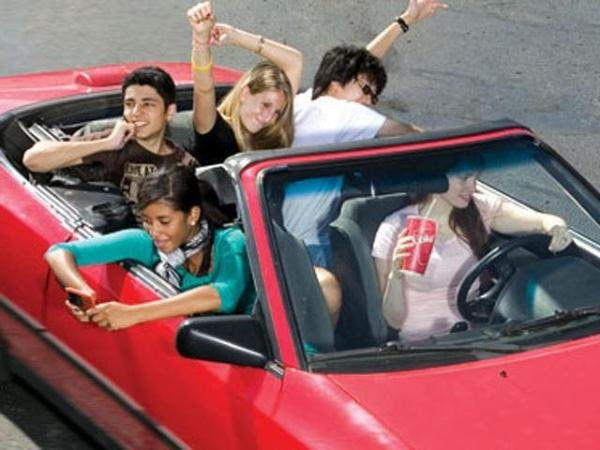
\includegraphics[width = 8cm]{images/new_car.jpg}
    	\end{figure}
\end{frame}
    
    
    

        

        
\begin{frame}{Adempimenti}
	\transdissolve<1>
	\begin{figure}[ht!]
    		\centering
         		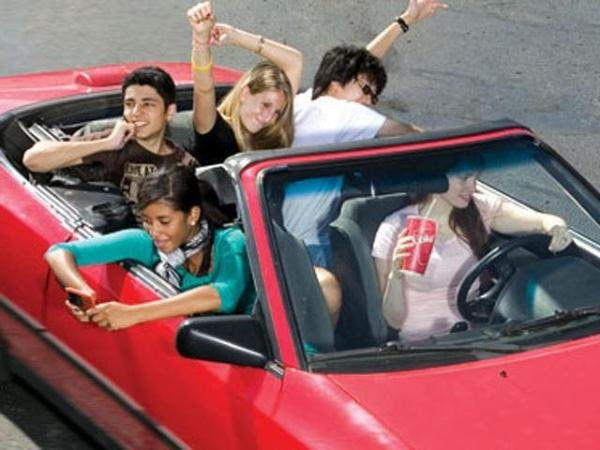
\includegraphics[width = 3cm]{images/new_car.jpg}
    	\end{figure}
    	Vai all'ACI di Prima Porta da Andrea. E' obbligatorio:
    	
    		\begin{enumerate}
    			\item<2-> PATENTE 		
   		 	\item<3-> IMMATRICOLAZIONE
    			\item<4-> ASSICURAZIONE
    			\item<5-> TRIANGOLO
    			\item<6-> Foglio rosa -> P
    		\end{enumerate}
\end{frame}
 
     
             
     
     
     
\begin{frame}{1. Patente}
	\begin{figure}[ht!]
    		\centering
         		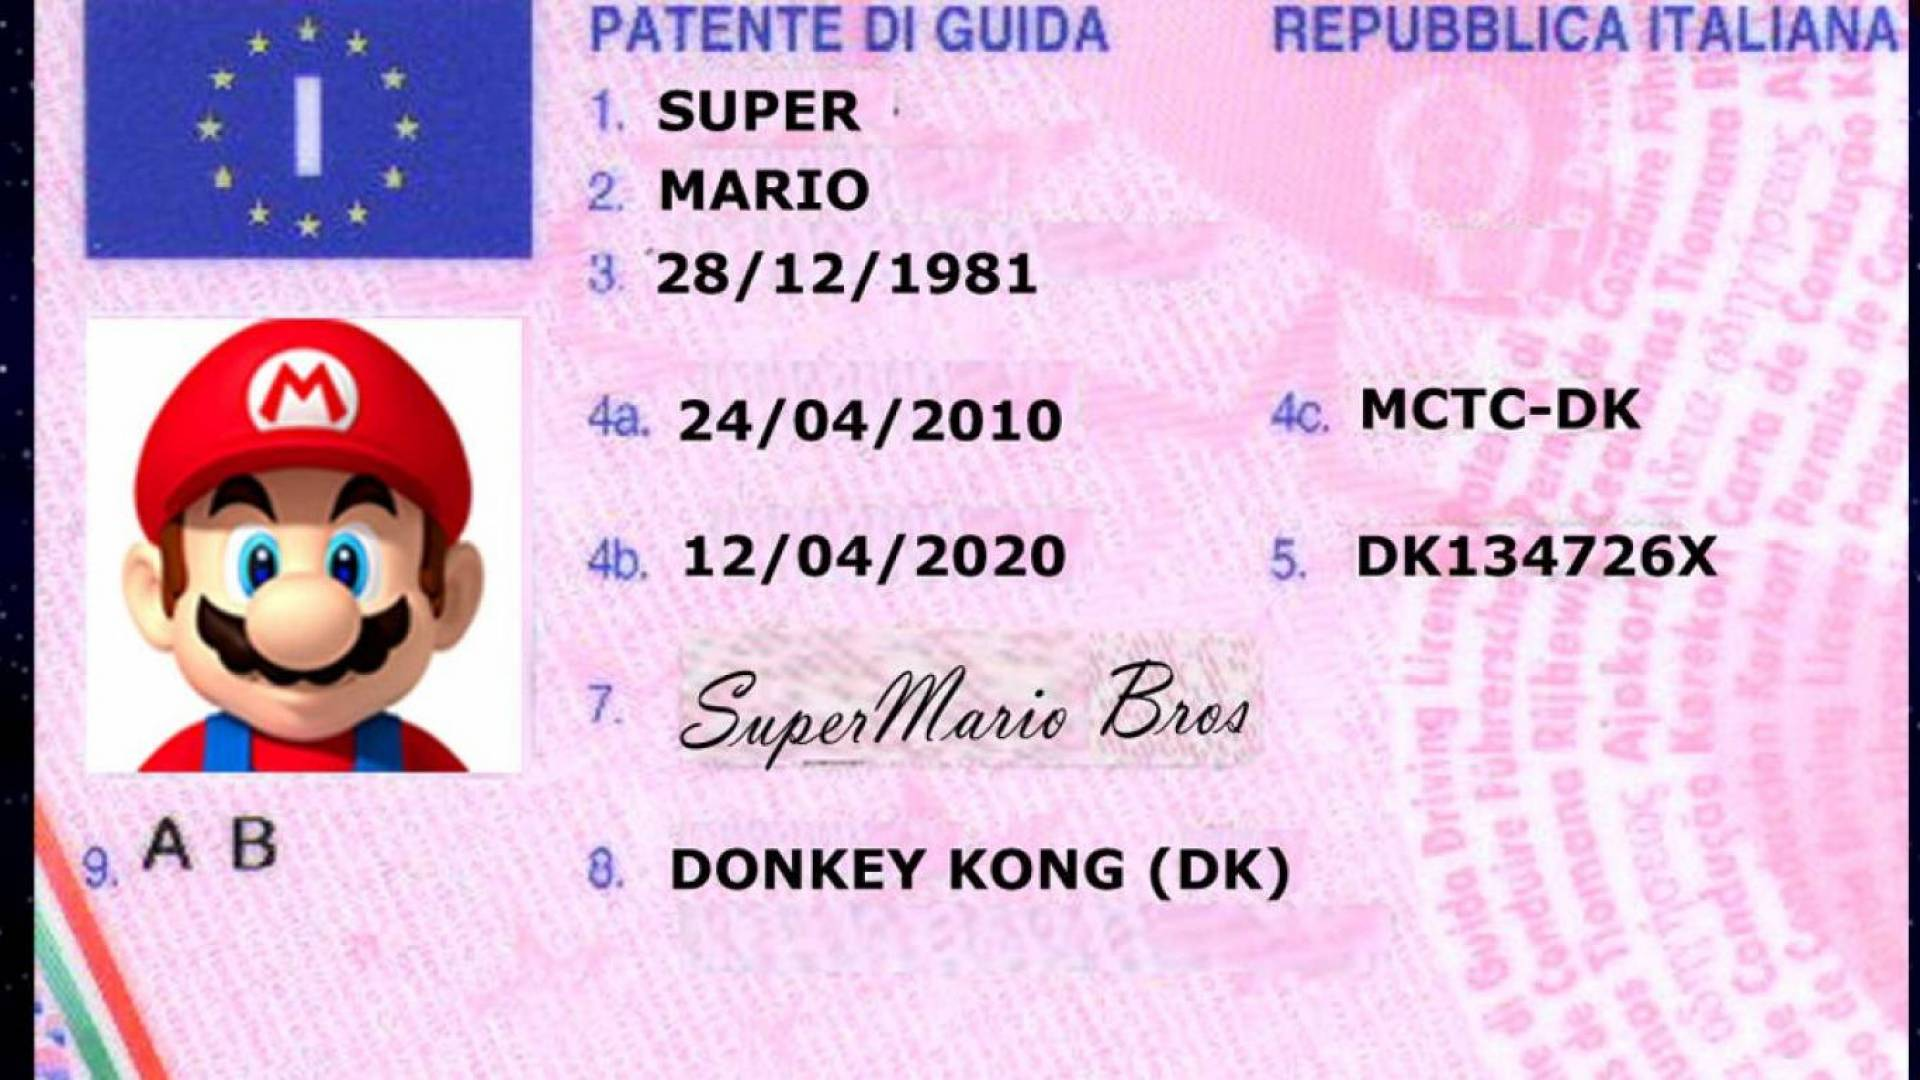
\includegraphics[width = 4cm]{images/patente.jpg}
    	\end{figure}
    	\begin{center}
    	\begin{tabular}{ |p{2cm}|p{7.2cm}|}
 \hline
 \multicolumn{2}{|c|}{\textbf{ Patenti sui quiz}} \\
 \hline
AM & ciclomotori\\
A1, A2, A& motocicli, tricicli, macchine agricole non eccezionali\\
B1& quadricicli\\
B & autoveicoli fino a 3,5 ton di peso e  max 9 persone\\
B96, BE & B+rimorchio\\
 \hline
\end{tabular}
\end{center}
\end{frame}     
    
    
    
\begin{frame}{2. Immatricolazione}
	\begin{figure}[ht!]
    		\centering
         		
\includegraphics[width = 3cm]{images/targa.jpg}
         		\hspace{1cm}
         		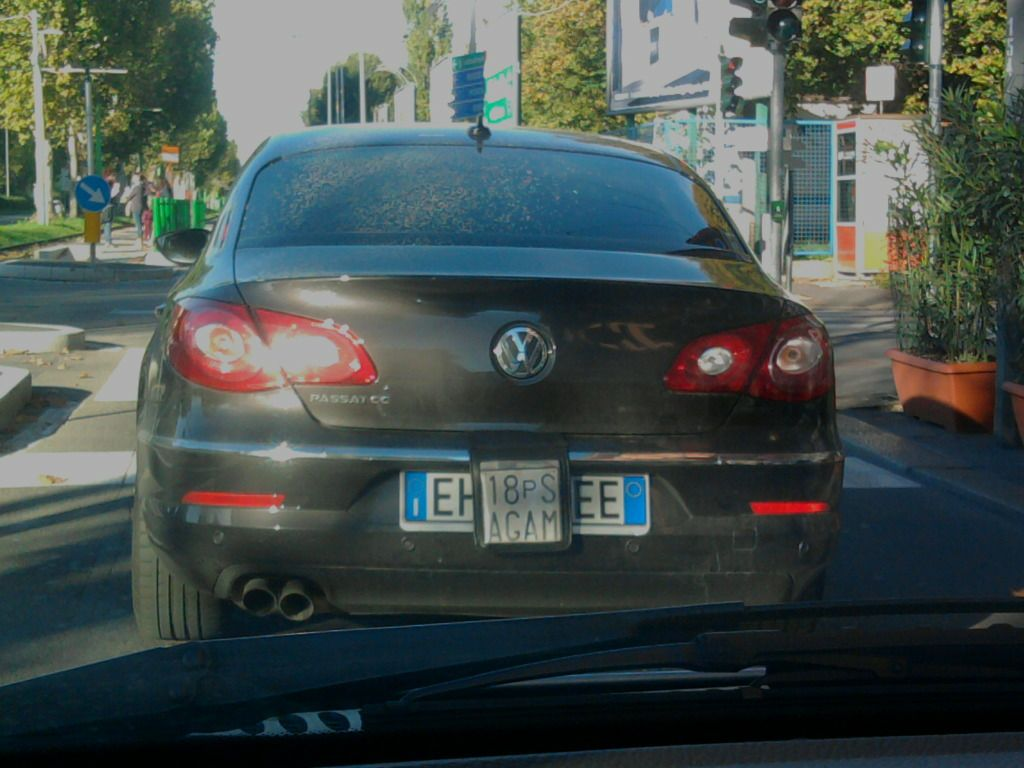
\includegraphics[width = 3cm]{images/targa_prova.jpg}
         		
         		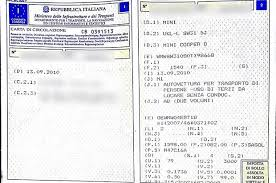
\includegraphics[width = 6cm]{images/libretto.jpg} 		
    	\end{figure}
\end{frame}  
    
  
  
    
\begin{frame}{3. Assicurazione}
	\begin{figure}[ht!]
    		\centering
         		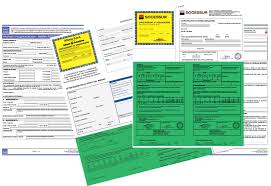
\includegraphics[width = 6cm]{images/assicurazione.jpg}
    	\end{figure}
\end{frame}       
        
        
        
\begin{frame}{4. TRIANGOLO}
	\begin{figure}[ht!]
    		\centering
         		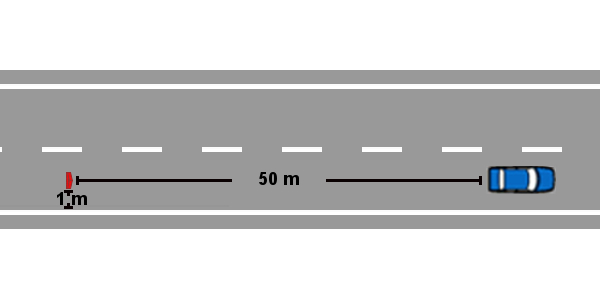
\includegraphics[width = 9cm]{images/triangolo.jpg}
    	\end{figure}
\end{frame} 

        
                 
\begin{frame}{5. FOGLIO ROSA}
	\begin{figure}[ht!]
    		\centering
         		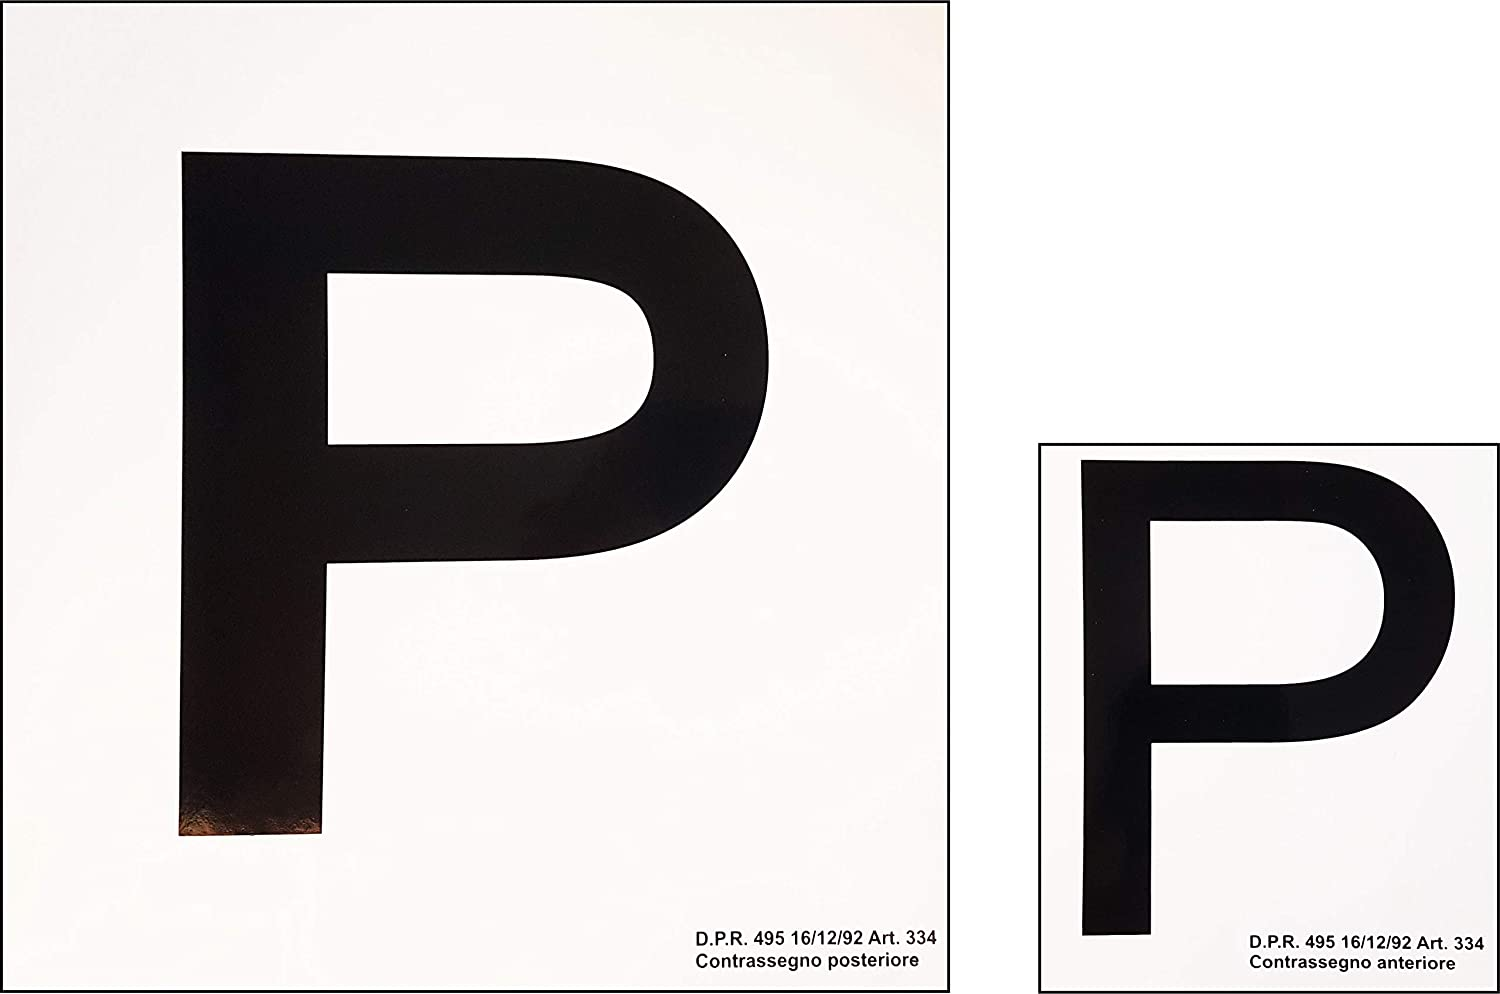
\includegraphics[width = 5cm]{images/p.jpg}
    	\end{figure}
\end{frame}               
            
    
\begin{frame}{Quiz 1}
	E' \only<1>{di norma} \only<2->{\alert{di norma}} vietato condurre sulle strade pubbliche un
	autoveicolo non immatricolato
     	
     	\quizV
        
\end{frame}
         
    
    
    
    
    
\begin{frame}{Quiz 2}
	E' vietato circolare sulle strade pubbliche con un autoveicolo dotato della targa prova
     
	\quizF
         
\end{frame}
    
    
    
    
    
    
\begin{frame}{Quiz 3}
	E' vietato utilizzare un autoveicolo sulle strade pubbliche quando non si ha con se la ricevuta di
	avvenuto pagamento della tassa di possesso
     
	\quizF
         
\end{frame}  
    
    
    
    
    
    
\begin{frame}{Quiz 4}
	 Sulle strade pubbliche \`e vietato utilizzare un autoveicolo se la garanzia \`e scaduta di validit\`a
     
	\quizF
         
\end{frame}      

  
    



  
\section{Trasporto di persone ed oggetti}



\begin{frame}{Sporgenza Autoveicolo}
\begin{figure}[ht!]
    		\centering
         		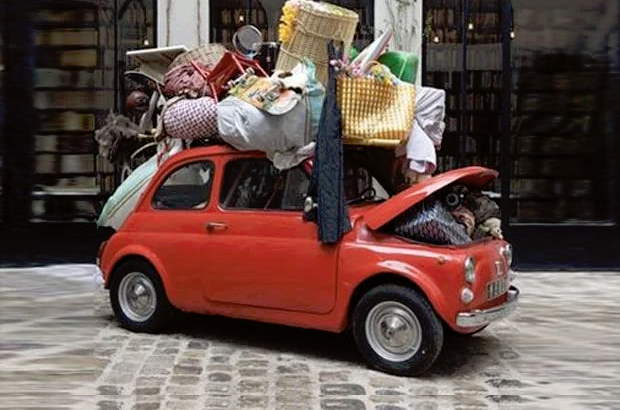
\includegraphics[width = 8cm]{images/esempio_sporg.png}
    	\end{figure}
\end{frame} 






\begin{frame}{Sporgenza Autoveicolo}
	\begin{figure}[ht!]
    		\centering
         		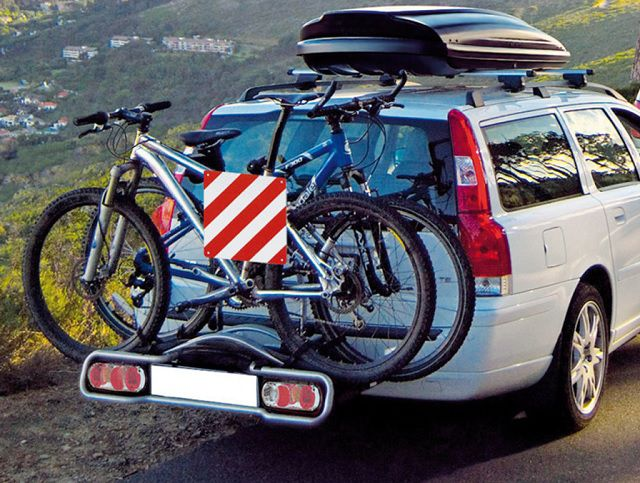
\includegraphics[width = 8cm]{images/esempio_sporgenza.jpg}
    	\end{figure}
\end{frame} 

    
    
    
    
\begin{frame}{Sporgenza Autoveicolo}
	\begin{figure}[ht!]
    		\centering
         		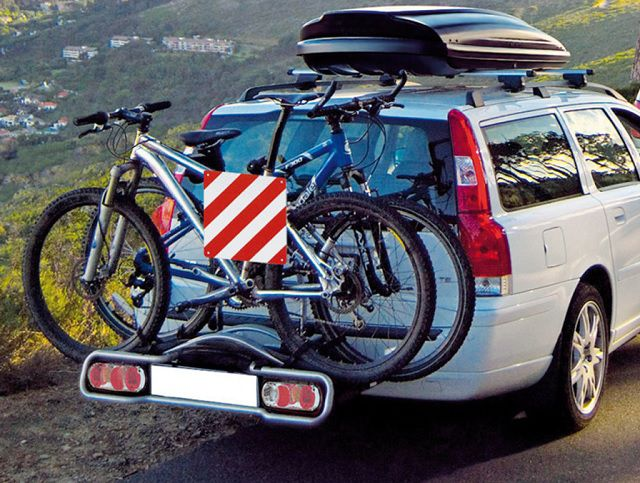
\includegraphics[width = 3cm]{images/esempio_sporgenza.jpg}
    	\end{figure}
    	\begin{description}
    	\item<1->[ - anteriore: ] \only<2->{NO}
    	\item<3->[- posteriore: ] \only<4->{3/10 lunghezza e  massimo 12m. 
    	\begin{animateinline}[autoplay,nomouse,loop]{1.4}
  \strut \alert{PANNELLO}\newframe[2.8] % [2.8] --> pause 1/2 as long as visible phase
\end{animateinline}
}
    	\item<5->[- laterale: ] \only<6->{30cm dalle luci}
    	\item<7->[- altezza: ] \only<8->{massimo 4m}
    	\end{description}
\end{frame} 
    
\end{document}
